\documentclass[a4paper,14pt]{extreport}
\usepackage[left=1.5cm,right=1.5cm,
    top=1.5cm,bottom=2cm,bindingoffset=0cm]{geometry}
\usepackage{scrextend}
\usepackage[T1,T2A]{fontenc}
\usepackage[utf8]{inputenc}
\usepackage[english,russian,ukrainian]{babel}
\usepackage{tabularx}
\usepackage{amssymb}
\usepackage{color}
\usepackage{amsmath}
\usepackage{mathrsfs}
\usepackage{listings}
\usepackage{graphicx}
\graphicspath{ {./images/} }
\usepackage{lipsum}
\usepackage{xcolor}
\usepackage{hyperref}
\usepackage{tcolorbox}
\usepackage{tikz}
\usepackage[framemethod=TikZ]{mdframed}
\usepackage{wrapfig,boxedminipage,lipsum}
\mdfdefinestyle{MyFrame}{%
linecolor=blue,outerlinewidth=2pt,roundcorner=20pt,innertopmargin=\baselineskip,innerbottommargin=\baselineskip,innerrightmargin=20pt,innerleftmargin=20pt,backgroundcolor=gray!50!white}
 \usepackage{csvsimple}
 \usepackage{supertabular}
\usepackage{pdflscape}
\usepackage{fancyvrb}
%\usepackage{comment}
\definecolor{ggreen}{rgb}{0.4,1,0}
\definecolor{rred}{rgb}{1,0.1,0.1}
\definecolor{aquamarine}{rgb}{0.5, 1.0, 0.83}
\definecolor{amber}{rgb}{1.0, 0.75, 0.0}
\definecolor{babyblue}{rgb}{0.54, 0.81, 0.94}
\usepackage{array,tabularx}
\usepackage{colortbl}

\usepackage{varwidth}
\tcbuselibrary{skins}
\usepackage{fancybox}

\usetikzlibrary{calc}
\makeatletter
\newlength{\mylength}
\xdef\CircleFactor{1.1}
\setlength\mylength{\dimexpr\f@size pt}
\newsavebox{\mybox}
\newcommand*\circled[2][draw=blue]{\savebox\mybox{\vbox{\vphantom{WL1/}#1}}\setlength\mylength{\dimexpr\CircleFactor\dimexpr\ht\mybox+\dp\mybox\relax\relax}\tikzset{mystyle/.style={circle,#1,minimum height={\mylength}}}
\tikz[baseline=(char.base)]
\node[mystyle] (char) {#2};}
\makeatother




\usepackage{float}
\usepackage{wrapfig}
\usepackage{framed}
%for nice Code{
\lstdefinestyle{customc}{
  belowcaptionskip=1\baselineskip,
  breaklines=true,
  frame=L,
  xleftmargin=\parindent,
  language=C,
  showstringspaces=false,
  basicstyle=\small\ttfamily,
  keywordstyle=\bfseries\color{green!40!black},
  commentstyle=\itshape\color{purple!40!black},
  identifierstyle=\color{blue},
  stringstyle=\color{orange},
}
\lstset{escapechar=@,style=customc}
%}
\usepackage{adjustbox}
\setlength{\parindent}{0pt}% Just for this example

\begin{document}
\pagecolor{white}
\begin{titlepage}
  \begin{center}
    \large
    Національний технічний університет України \\ "Київський політехнічний інститут імені Ігоря Сікорського"


    Факультет Електроніки

    Кафедра мікроелектроніки
    \vfill

    \textsc{ЗВІТ}\\

    {\Large Про виконання лабораторної роботи №2\\
      з дисципліни: «Вакуумна та плазмова електроніка»\\[1cm]

       ГАЗОРОЗРЯДНІ ЛАМПИ


    }
  \bigskip
\end{center}
\vfill

\newlength{\ML}
\settowidth{\ML}{«\underline{\hspace{0.4cm}}» \underline{\hspace{2cm}}}
\hfill
\begin{minipage}{1\textwidth}
Виконавець:\\
Студент 3-го курсу \hspace{4cm} $\underset{\text{(підпис)}}{\underline{\hspace{0.2\textwidth}}}$  \hspace{1cm}Б.\,В.~Лищенко\\


Перевірив: \hspace{5.9cm} $\underset{\text{(підпис)}}{\underline{\hspace{0.2\textwidth}}}$  \hspace{1cm}О.\,М.~Бевза\\

\end{minipage}

\vfill

\begin{center}
2021
\end{center}
\end{titlepage}



\textbf{Мета роботи}: Дослідити роботу газорозрядної лампи, а також процеси, що приймають участь в передачі енергії в газорозрядних лампах.
\begin{center}\textbf{Завдання}\end{center}\par
\newtcbox{\xmybox}[1][red]{on line, arc=7pt,colback=#1!10!white,colframe=#1!50!black, before upper={\rule[-3pt]{0pt}{10pt}},boxrule=1pt, boxsep=0pt,left=6pt,right=6pt,top=2pt,bottom=2pt}

\begin{enumerate}
\item Запустіть програму «Неонова та інші газорозрядні лампи.jar» та ознайомтесь з елементами керування програмою.\\

\item Виберіть закладку «Один атом». В списку, що розкривається, «Хімічний 
елемент» виберіть «Налаштовуваний».\\

\item Ви можете вибрати кількість порожніх електронних рівнів енергії в 
конфігуруваному атомі та відрегулювати їх розташування, а також ви можете 
переміщати атом в розрядній трубці.\\

\item Виберіть закладку «Багато атомів».
\item У вікні «Випроміненя електронів» виберіть «Неперервне». Діапазон у \% 
можна встановити за вашим бажанням.
\item Праворуч на екрані, в списку, що розкривається, «Хімічний елемент», почніть 
з Водню.
\item У нижньому правому куті, у полі “Описання” натисніть на Спектрометр.
\item Запустивши процес моделювання, почекайте коли одна з ліній спектру набуде 
максимального значення і зафіксуйте спектр. Вкажіть лінії спектру (довжину 
випромінювання) і їх процентне співвідношення в загальному спектрі 
випромінювання водню. 
\item Змінюючи напругу прискорення визначити мінімальну напругу виникнення 
світіння в газорозрядній трубці для водню. Як напруга прискорення впливає 
на спектр випромінювання газорозрядної трубки?
\item Повторити пункти 10 та 11 для Ртуті, Натрію та Неону
\end{enumerate}
\newpage
%-----------------------------------------------------------------------------------------------------------------------------------1
\begin{center}
Виконання роботи
\end{center}


	




\begin{center}\fcolorbox{black}{babyblue}{Водень}
 
 
		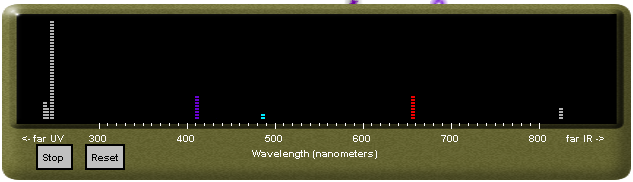
\includegraphics[width=0.7\linewidth]{1.png}\end{center}

	\begin{center}
		\begin{tabular}{|c|c|}
		\hline
		\multicolumn{2}{|c|}{18 В}                              \\ \hline
		                             & \%                       \\ \hline
		UV1                          & 11                   \\ \hline
		UV2                          & 56                   \\ \hline
		IR                           & 7                     \\ \hline
		405 нм                       & 16                      \\ \hline
		485 нм                       & 3                      \\ \hline
		655 нм                       & 13						\\ \hline
		\end{tabular}
	\end{center}





%-----------------------------------------------------------------------------------------------------------------------------------2


%\clipbox{0 0 0 \dimexpr\height-10pt}{
\includegraphics[width=\linewidth]{111.png}}

\begin{center}\fcolorbox{black}{babyblue}{Ртуть}


		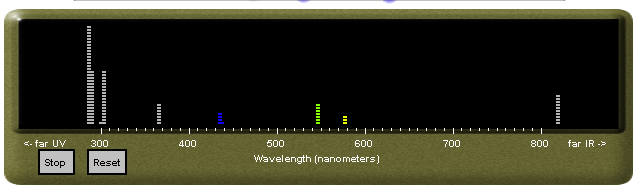
\includegraphics[width=0.7\linewidth]{2.png}\end{center}

	\begin{center}
		\begin{tabular}{|c|c|}
		\hline
		\multicolumn{2}{|c|}{18 В}                              \\ \hline
		                             & \%                       \\ \hline
		UV1                          & 51                   \\ \hline
		IR                           & 5                     \\ \hline
		300 нм                       & 22                      \\ \hline
		445 нм                       & 4                      \\ \hline
		365 нм                       & 5                      \\ \hline
		545 нм                       & 9                      \\ \hline
		575 нм                       & 3						\\ \hline
		\end{tabular}
	\end{center}

\newpage


%-----------------------------------------------------------------------------------------------------------------------------------3
 
\begin{center}\fcolorbox{black}{babyblue}{Натрій}
 

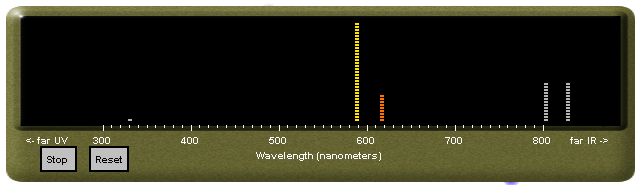
\includegraphics[width=0.7\linewidth]{3.png}\end{center}

		\begin{center}
	%\caption{Натрій}
		\begin{tabular}{|c|c|}
		\hline
		\multicolumn{2}{|c|}{18 В}                              \\ \hline
		                             & \%                       \\ \hline
		IR1                          & 14                     \\ \hline
		IR2                          & 16                      \\ \hline
		330 нм                       & 4                     \\ \hline
		590 нм                       & 46                      \\ \hline
		620 нм                       & 20                     \\ \hline
		\end{tabular}
	\end{center}

 

 






%-----------------------------------------------------------------------------------------------------------------------------------4
		\begin{center}\fcolorbox{black}{babyblue}{Неон}
		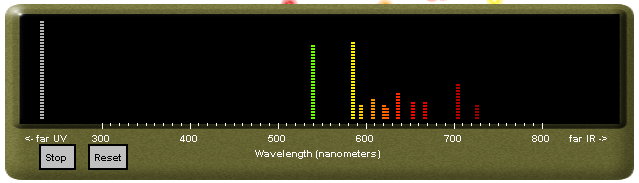
\includegraphics[width=0.7\linewidth]{4.png}\end{center}

	\begin{center}
	%\caption{Неон}
		\begin{tabular}{|c|c|}
		\hline
		\multicolumn{2}{|c|}{30 В}                              \\ \hline
		                             & \%                       \\ \hline
		UV                       & 27                   \\ \hline
		540 нм                       & 17                      \\ \hline
		585 нм                       & 18                    \\ \hline
		595 нм                       & 2                      \\ \hline
		610 нм                       & 6                    \\ \hline
		620 нм                       & 4                      \\ \hline
		635 нм                       & 5                    \\ \hline
		655 нм                       & 3                    \\ \hline
		665 нм                       & 3                    \\ \hline
		710 нм                       & 6                    \\ \hline
		725 нм                       & 2                     \\ \hline
		\end{tabular}
	\end{center}


\clearpage
\newpage
\begin{enumerate}
	\item Якщо відстань між двома електронними енергетичними рівнями в атомі 
	А більше, ніж в атомі В, тоді довжина хвилі світла, випромінюваного 
	атомом В, буде більше; --- так
	\item Якщо відстань між двома електронними енергетичними рівнями в атомі 
	А менше, ніж в атомі В, тоді атом Б буде випромінювати фотони з 
	меншою енергією; ---  так
	\item Фотони випромінюються, коли електрони в атомі набувають енергію; --- ні
	\item Кольори, які випромінює атом, залежать від того, скільки кінетичної 
	енергії має вільний електрон, потрапляючи на атом;
	--- ні
	\item Кольори, що випромінюються, залежать від кількості вільних 
	електронів, що проходять через лампу;
	--- ні
	\item Коли вільний електрон потрапляє на атом, атом завжди збуджується до 
	максимально можливого енергетичного рівня;
	--- так
	\item Кінетична енергія вільного електрона в точці зіткнення зростає зі 
	збільшенням напруги батареї;
	--- ні
	\item Кінетична енергія вільного електрона в точці зіткнення вища, якщо атом 
	знаходиться ближче до джерела електронів;
	--- ні
	\item Єдиний спосіб випромінювати ІЧ-фотони – це якщо порожні електронні 
	рівні енергії дійсно близькі до основного стану (найнижчий рівень 
	енергії);
	--- так
	\item Коли атомні електрони збуджуються на більш високий рівень, вони 
	завжди повертаються до свого найнижчого енергетичного рівня, 
	стрибаючи по одному за раз.
	--- ні
	\item Скільки можливих кольорів може випромінювати атом з 6 
	електронними рівнями енергії (основний стан – 6-й, найнижчий)?
	--- 6
	\item Що означає термін «збуджений»?\\
	це електрон який набувши додадткової
		енергiї, переходить у неосновний стан, на бiльш високий рiвень.
	\item Як атоми в імітованій трубці збуджуються?\\
	збуджнеея атомыв, якi знаходилися близько до електроду, з якого емiтували	електрони, майже не відбувалось.
	\item Що має статися, щоб збуджені атоми випускали фотони?\\
	треба щоб збуджений електрон повернувся у свiй основний рiвень енергiї.
	\item Чому фотони відображаються як різні кольори?\\
	колiр фотону залежить вiд кiлькостi енергетичних рiвнiв, якi в ньому знаходяться.
\end{enumerate}









\textbf{Висновок}: в цій лабораторній роботі було досліджено роботу газорозрядніх ламп та процеси, що приймають участь в передачі енергії в них, 

за допомогою симулятора лампи  були виведени на екран спектральні лінії на різноманітних довжинах хвиль, в залежності від газу який наповнював лампу. Після аналізу можна сказати, що найбільша частина значень припадає для водню та ртуті припадає на УФ, для натрію та неону -- жовта и помаранчова частини спектру, а для неону -- зелена та червона частина спектру.
















\end{document}
